\documentclass[border=10pt]{standalone}
\usepackage{tkz-fct}
\usepackage{tkz-base}
\usepackage{array}

\begin{document}

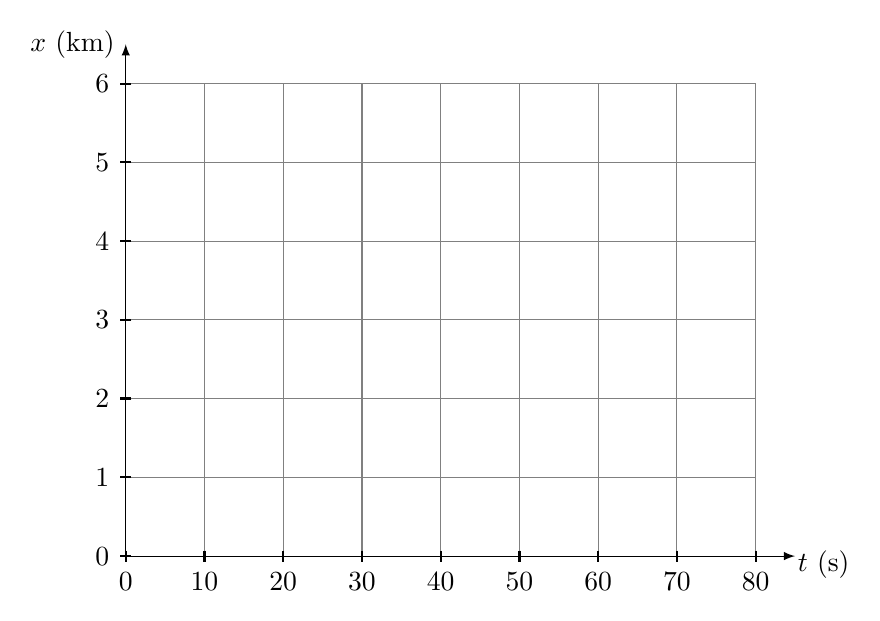
\begin{tikzpicture}
% Tableau en LaTeX standard avec tkz-text

% Repère quadrillé
\tkzInit[xmin=0,xmax=80,xstep=10,ymin=0,ymax=6, ystep=1]
\tkzGrid
\tkzDrawX[label = $t$ (s), right]
\tkzDrawY[label = $x$ (km)]
\tkzLabelXY
\tkzFct[line width=2pt, domain=0:80]{0.040*\x+2}


\end{tikzpicture}

\end{document}
